\documentclass[../main.tex]{subfiles}

\begin{document}
    \subsection{Predstavenie riešiteľského kolektívu}   
    Na riešení projektu sa podieľali nasledovní študenti:

        Bc. Eva Štalmachová - študentka inžinierského študijného programu Robotika a Kybernetika na Ústave Robotiky a Kybernetiky FEI STU

        Bc. Marek Trebuľa - študent inžinierského študijného programu Robotika a Kybernetika na Ústave Robotiky a Kybernetiky FEI STU

        Bc. Ján Urdianyk - študent inžinierského študijného programu Robotika a Kybernetika na Ústave Robotiky a Kybernetiky FEI STU

        Bc. Denis Vasko - študent inžinierského študijného programu Robotika a Kybernetika na Ústave Robotiky a Kybernetiky FEI STU

    \subsection{Plán projektu}   
    Vytvorili sme rozpis úloh na jednotlivé týždne semestra:
    \begin{enumerate}
    	\item Voľba témy. Určenie spôsobu komunikácie, dohodnutie stretnutí. 
    	\item Voľba vedúceho tímu, analýza problému, dohoda o obsahu riešenia. Zaučenie členov pre prácu s programom git. 
    	\item Štúdium literatúry zaoberajúcou sa danou problematikou.
    	\item Určenie prvotných úloh jednotlivých členov tímu.
    	\item Kontrola splnenia pridelených úloh, odvodenie ďalších úloh.
    	\item Dokumentácia vyriešených častí úlohy. A príprava prezentácie čiastočného riešenia.
    	\item Prezentácia čiastočného riešenia vedúcemu projektu, analýza kritiky vedúceho a syntéza nových úloh. 
    	\item Riešenie a dokumentácia nových úloh, konzultácia s vedúcim projektu.
    	\item Pokračovanie v riešení úloh z predchádzajúceho týždňa.
    	\item Destilácia obsahu riešenia do formy prezentácie.
    	\item Vypracovanie posudku na konkurenčný projekt.
    	\item Prezentácia.
    \end{enumerate}

    \subsection{Dohodnuté metódy práce}   
    	\begin{itemize}
    		\item Pre projekt bude vytvorený repozitár na stránkach github.com, do ktorého bude každý z členov prispievať svoju časť riešenia.
    		\item Forma riešenia bude predpísaná šablónou, ktorou sa členovia budú riadiť pri štrukturovaní práce a dokumentácie.
            \item Dokumentácia bude vytvorená v dokumentačnom systéme LaTeX.
            \item Simulácie budú vytvorené v simulačnom prostredí Matlab/Simulink.
            \item Verzie riešenia budú spravované využitím programu git a jednotlivé verzie budú hostované na stránkach github.com ako súkromný repozitár.
            \item Pre zabezpečenie dodržania termínov sme zaviedli aj časové obmedzenia doby riešenia jednotlivých úloh pridelených členom skupiny.
    	\end{itemize}

    \subsection{Komunikácia a koordinácia projektu}
    	\begin{itemize}
            \item Komunikácia s pánom prof. Murgašom prebieha počas naplánovaných stretnutí, alebo mailom (neskôr prebiehala výlučne mailom).
    		\item Medzi členmi tímu prostredníctvom facebookovej skupiny, alebo osobne. 
            \item Neskôr väčšina komunikácie medzi členmi tímu prebiehala prostredníctvom programu MS teams, využitím textových správ ale aj videohovorov.
    	\end{itemize}

    \subsection{Kontrola rozhodnutí tímu}
    Rozhodnutia o forme riešenia sme robili v prvých týždňoch semestra. Uvažovali sme nad rôznymi rozdeleniami práce, ako aj nad tým, čo by v riešení malo byť. 

    Rozhodli sme predviesť každú metódu dvoma príkladmi. Čo umožňovalo priradiť každému členu tímu jeden príklad. Ukázalo sa, že to bolo dobré rozhodnutie, pretože takto mohli členovia tímu pracovať paralelne.

    Rozhodli sme sa vytvoriť ukážkovú aplikáciu v Matlabe, kde by bolo možné demonštrovať rozdieli medzi PID regulátorom a nelineárnymi regulátormi. Avšak rozhodnutie použiť Matlab na vývoj tejto aplikácie sa ukázalo ako zlé rozhodnutie, pretože viedlo na problémy s kompatibilitou verzií Matlabu a zbytočnej zložitosti pri spúštaní programu.

    Využitie programovacieho jazyka TeX a balíčka makier LaTeX na formátovanie dokumentácie bolo dobrým rozhodnutím, pretože sme sa nemuseli zaoberať napríklad manuálnym číslovaním obrázkov.

    Ukladanie čiastočných riešení do git repozitáru na internet, sa ukázalo ako efektívny spôsob zaručenia aktuálnosti verzií a zosúladenia zmien súborov projektu medzi členmi tímu.

    Zavedenie časových limitov (deadline), na dokončenie čiastočných úloh, viedlo, podľa nášho názoru, k výrazne vyššej produktivite. Čiže ich zavedenie bolo dobrým rozhodnutím.
    
    \subsection{Podrobné záznamy o stretnutí}
    Uvádzame vyhotovené zápisnice stretnutí, zápisnice vypracoval Bc. Marek Trebuľa.

    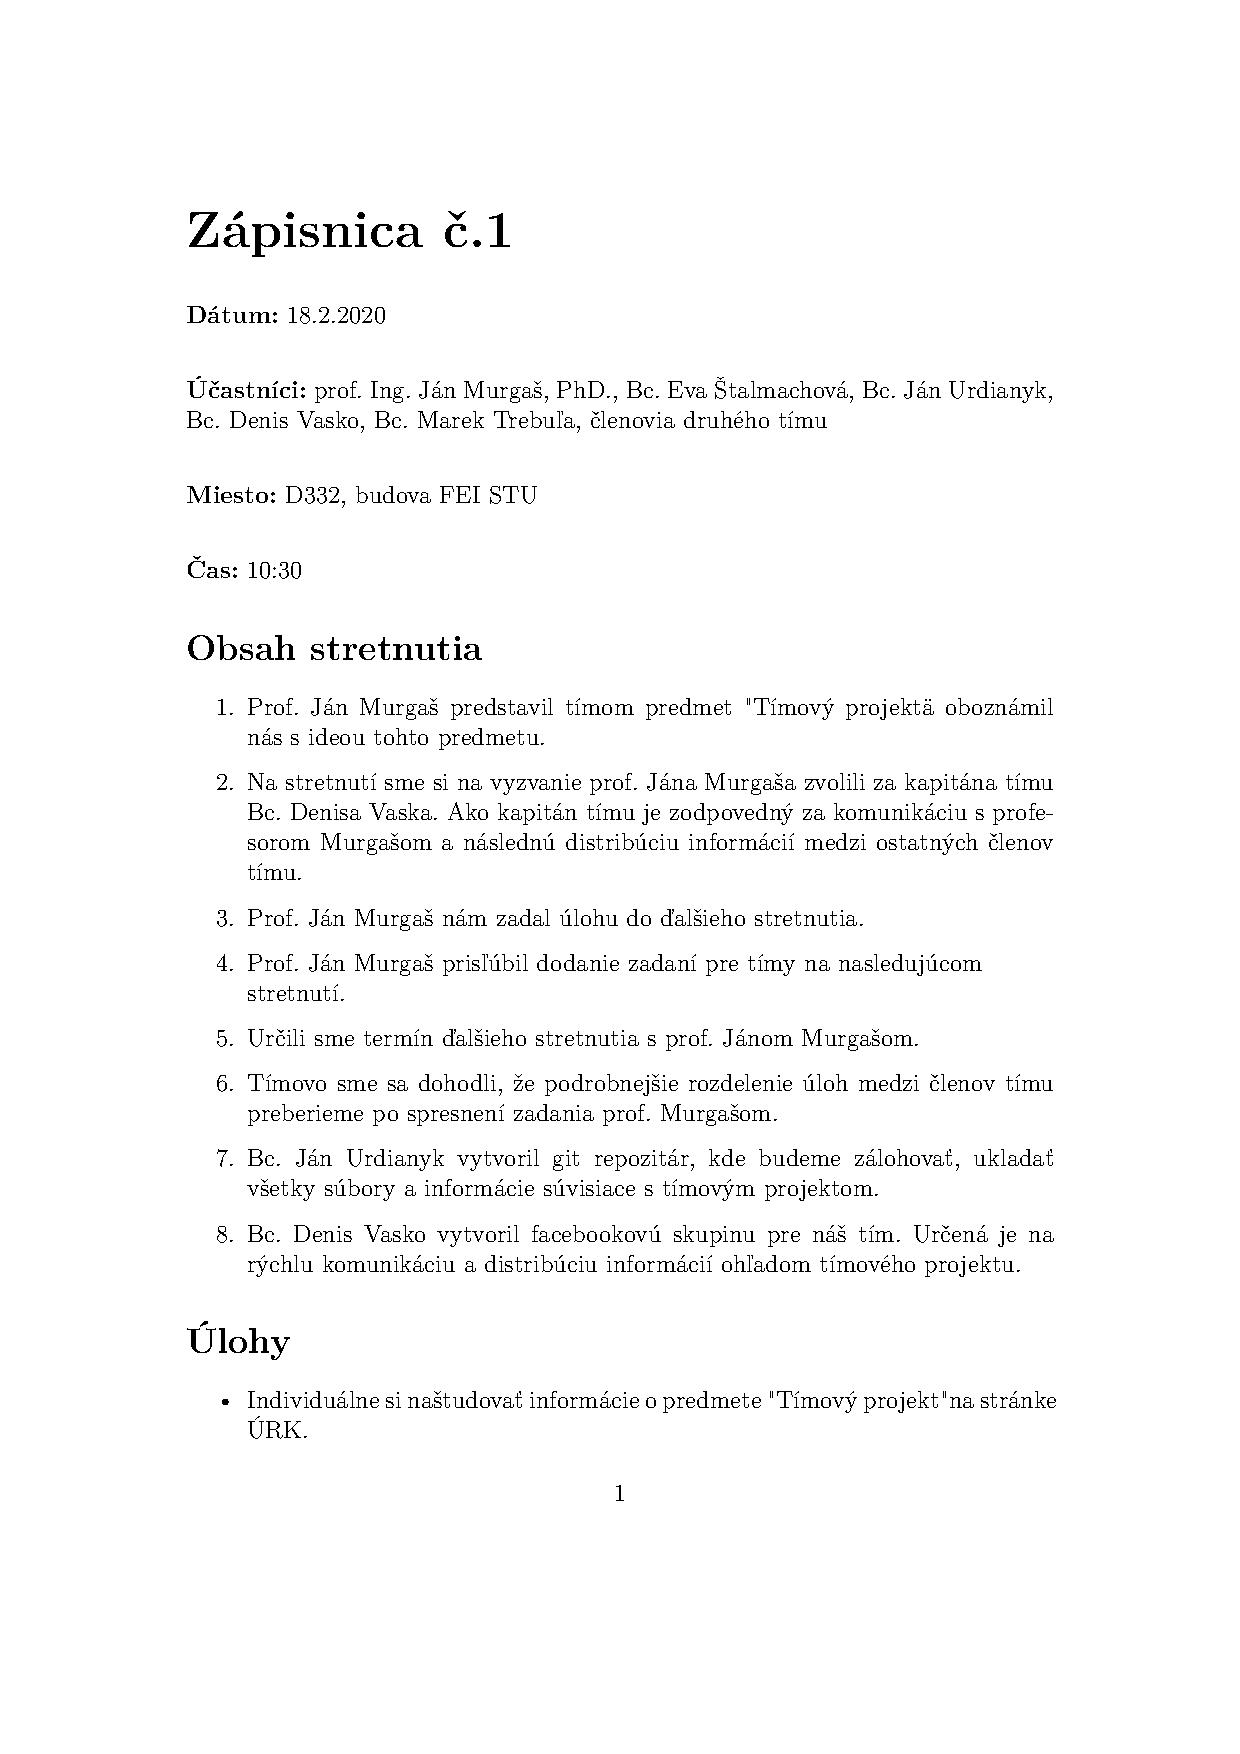
\includepdf{../../Zapisnice/Zapisnica1_18022020.pdf}
    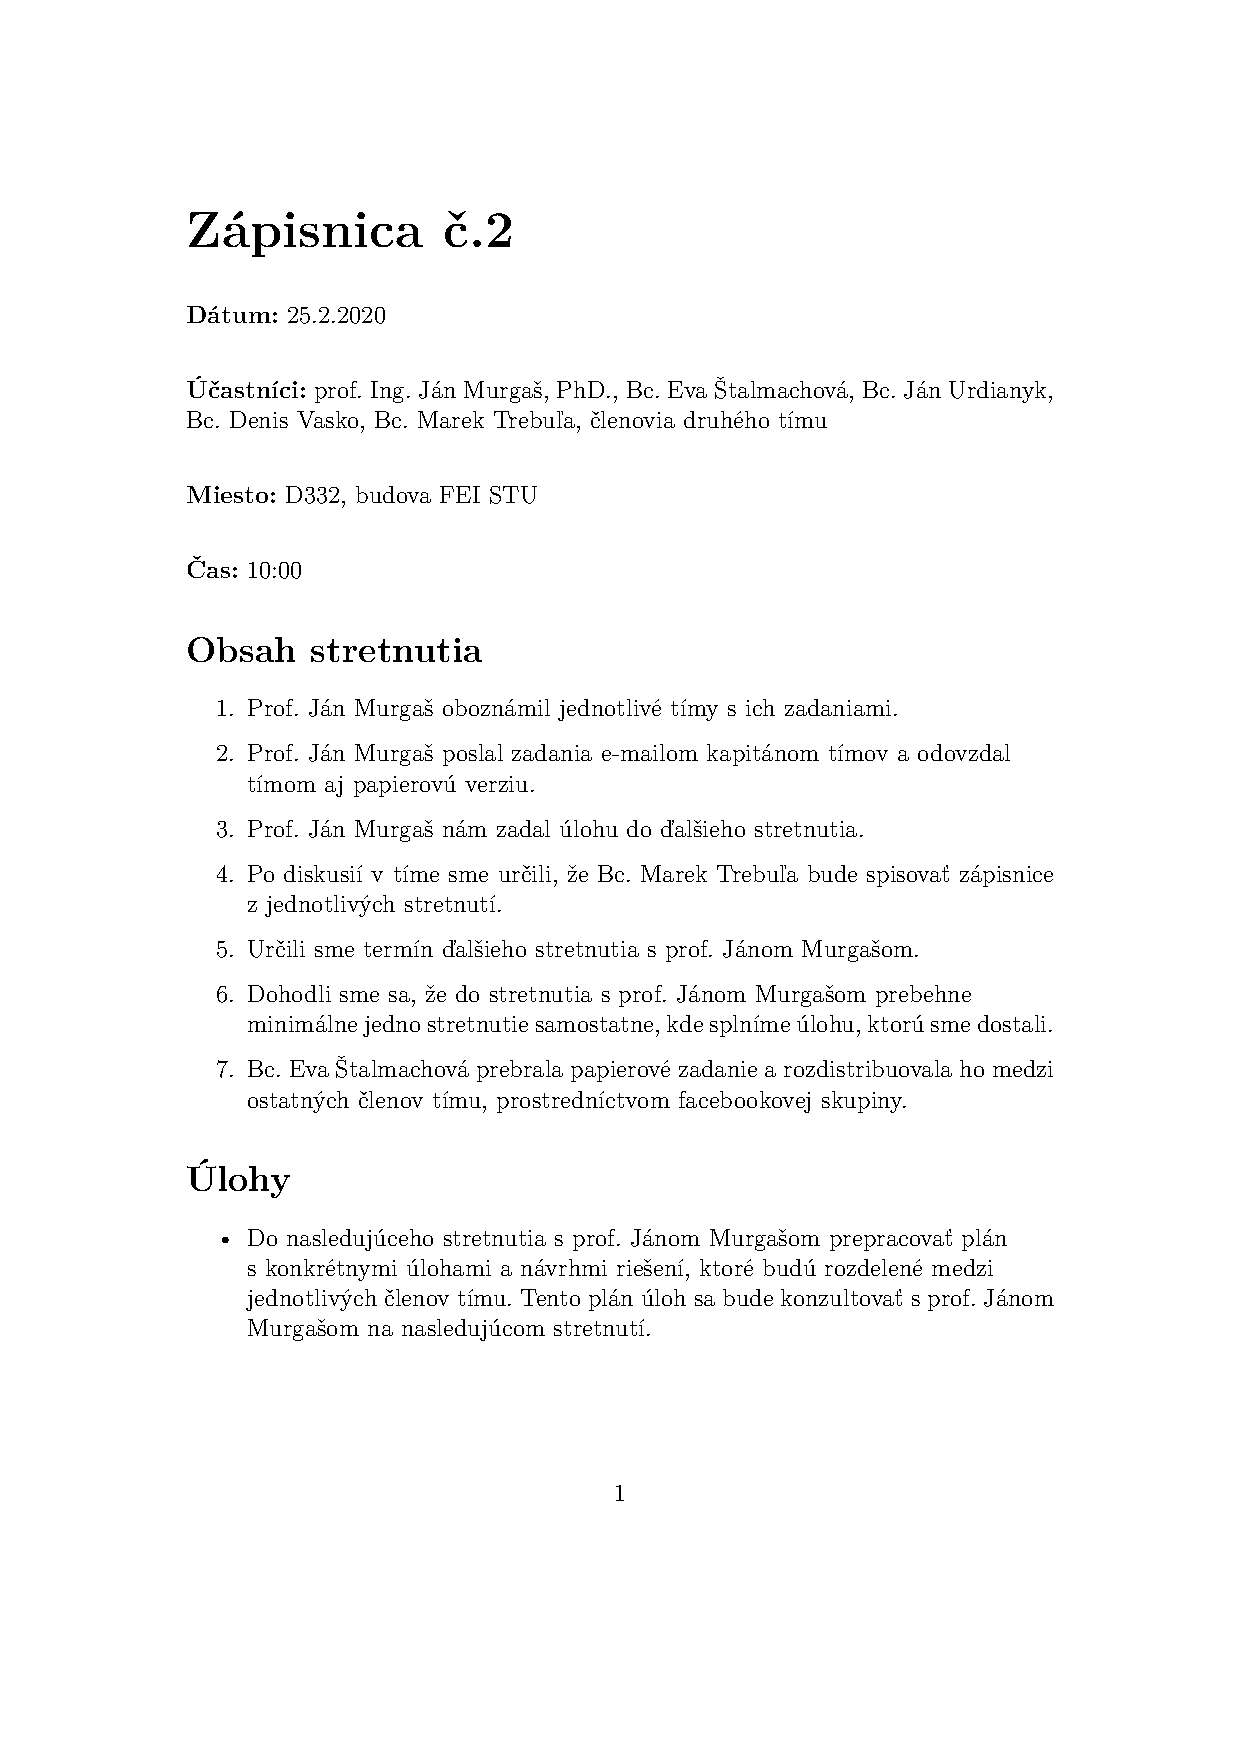
\includepdf{../../Zapisnice/Zapisnica2_25022020.pdf}
    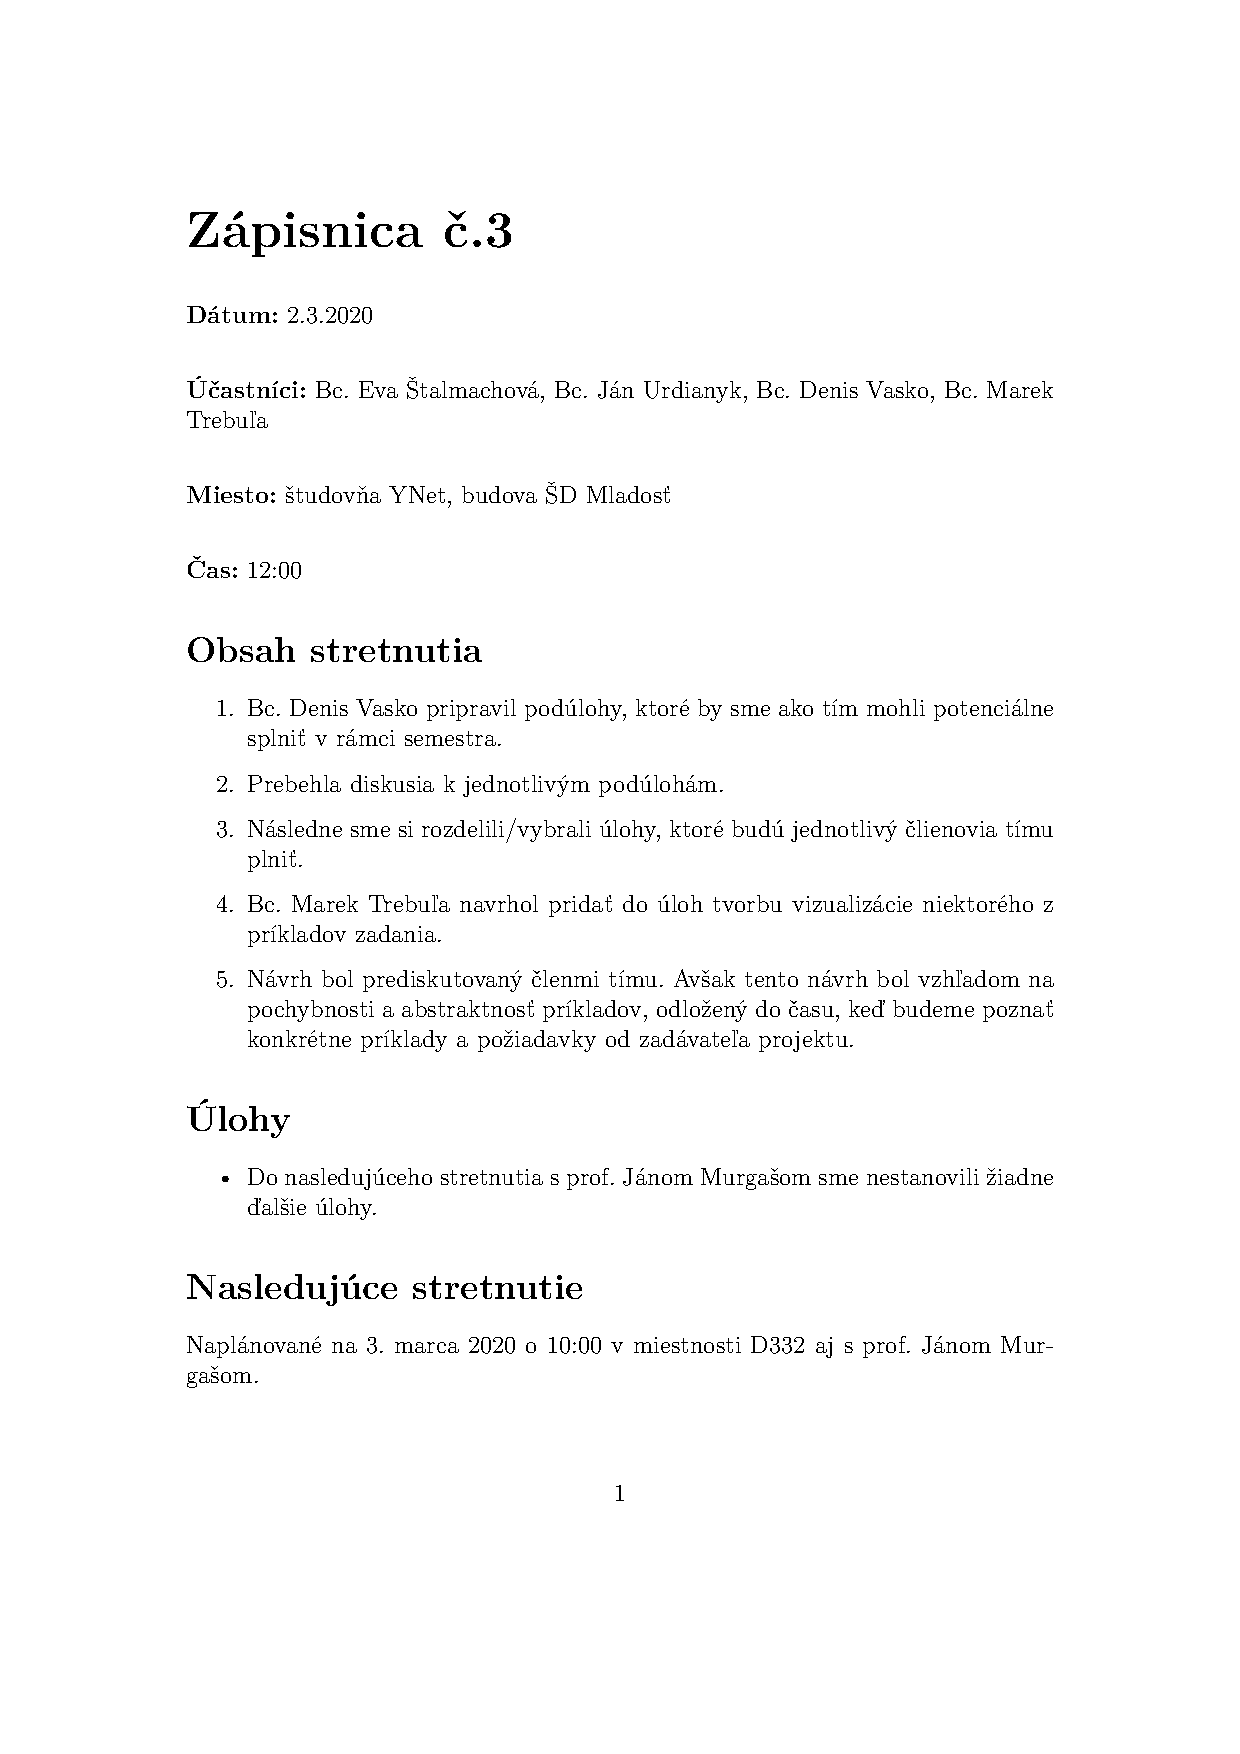
\includepdf{../../Zapisnice/Zapisnica3_02032020.pdf}
    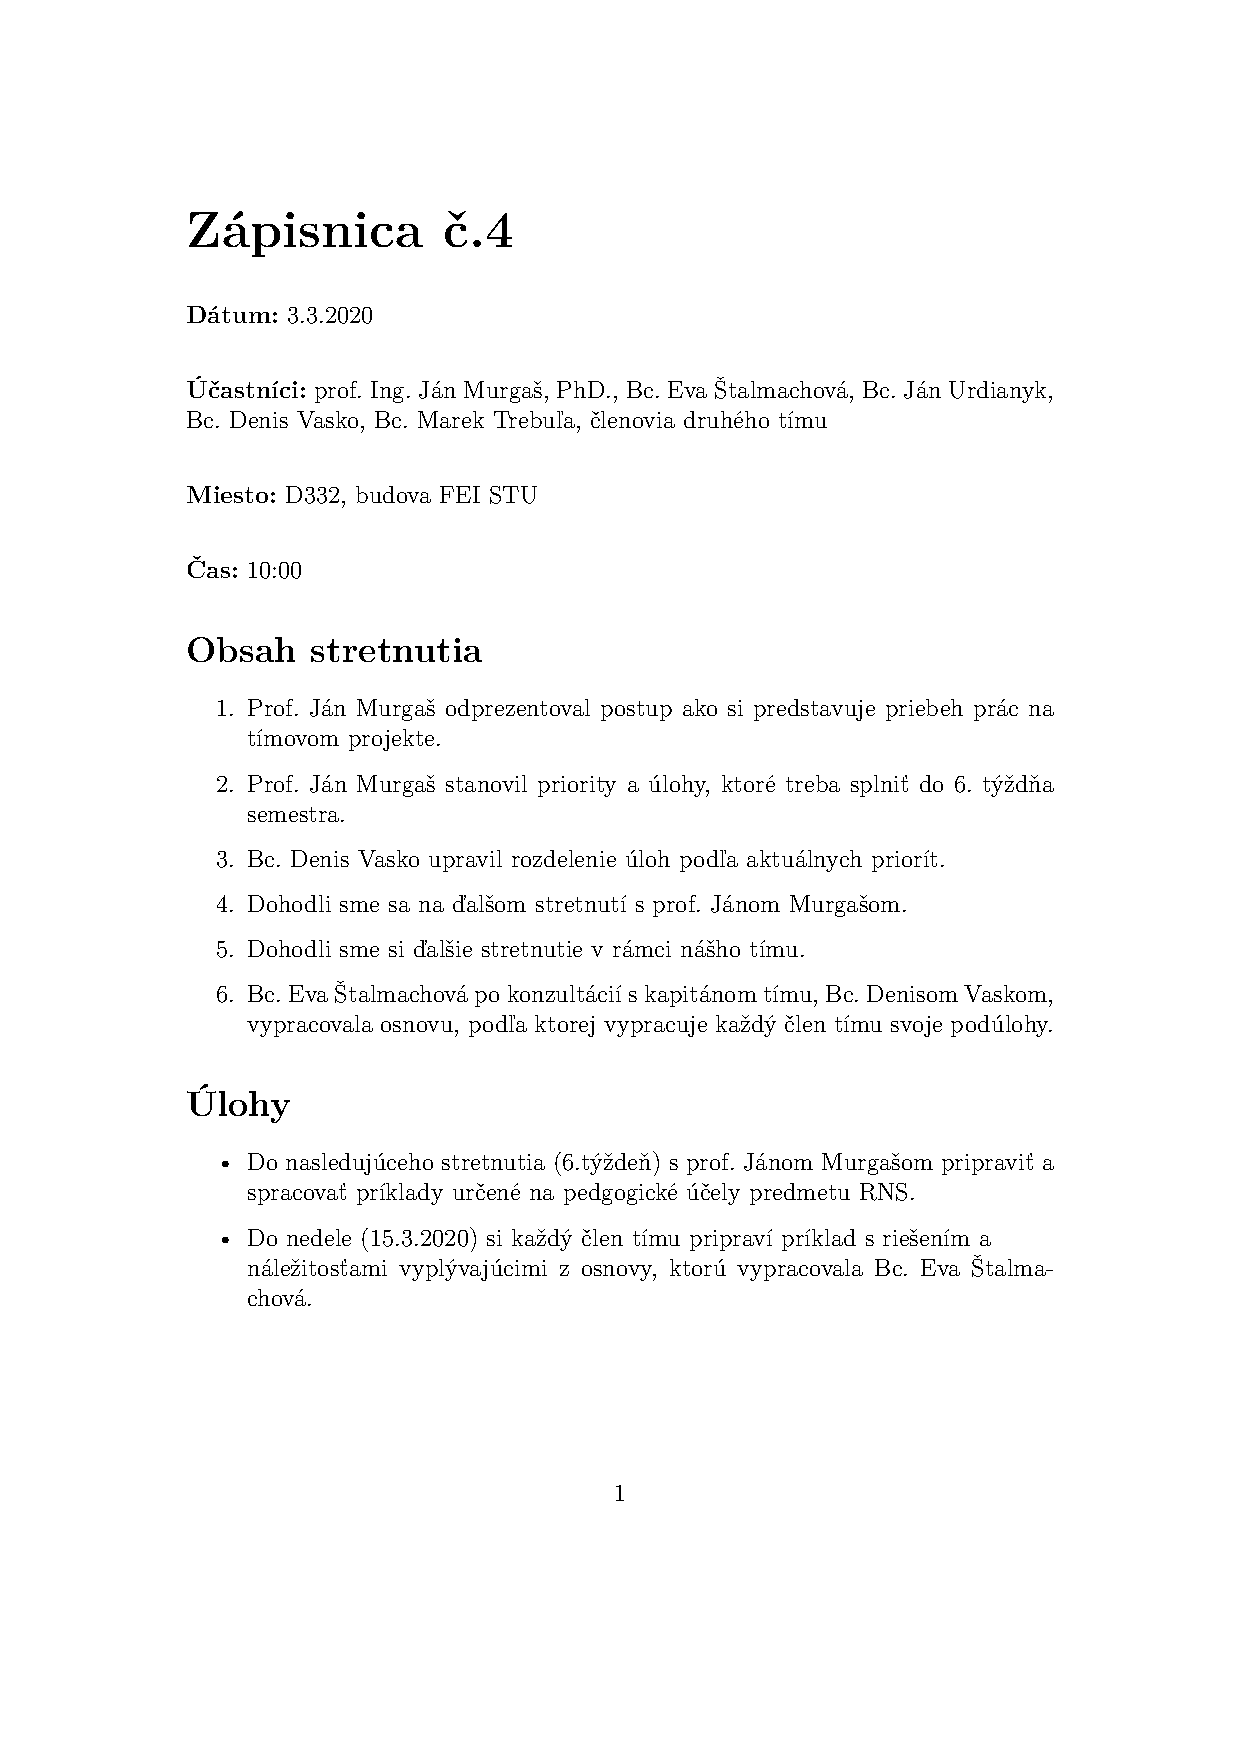
\includepdf{../../Zapisnice/Zapisnica4_03032020.pdf}
    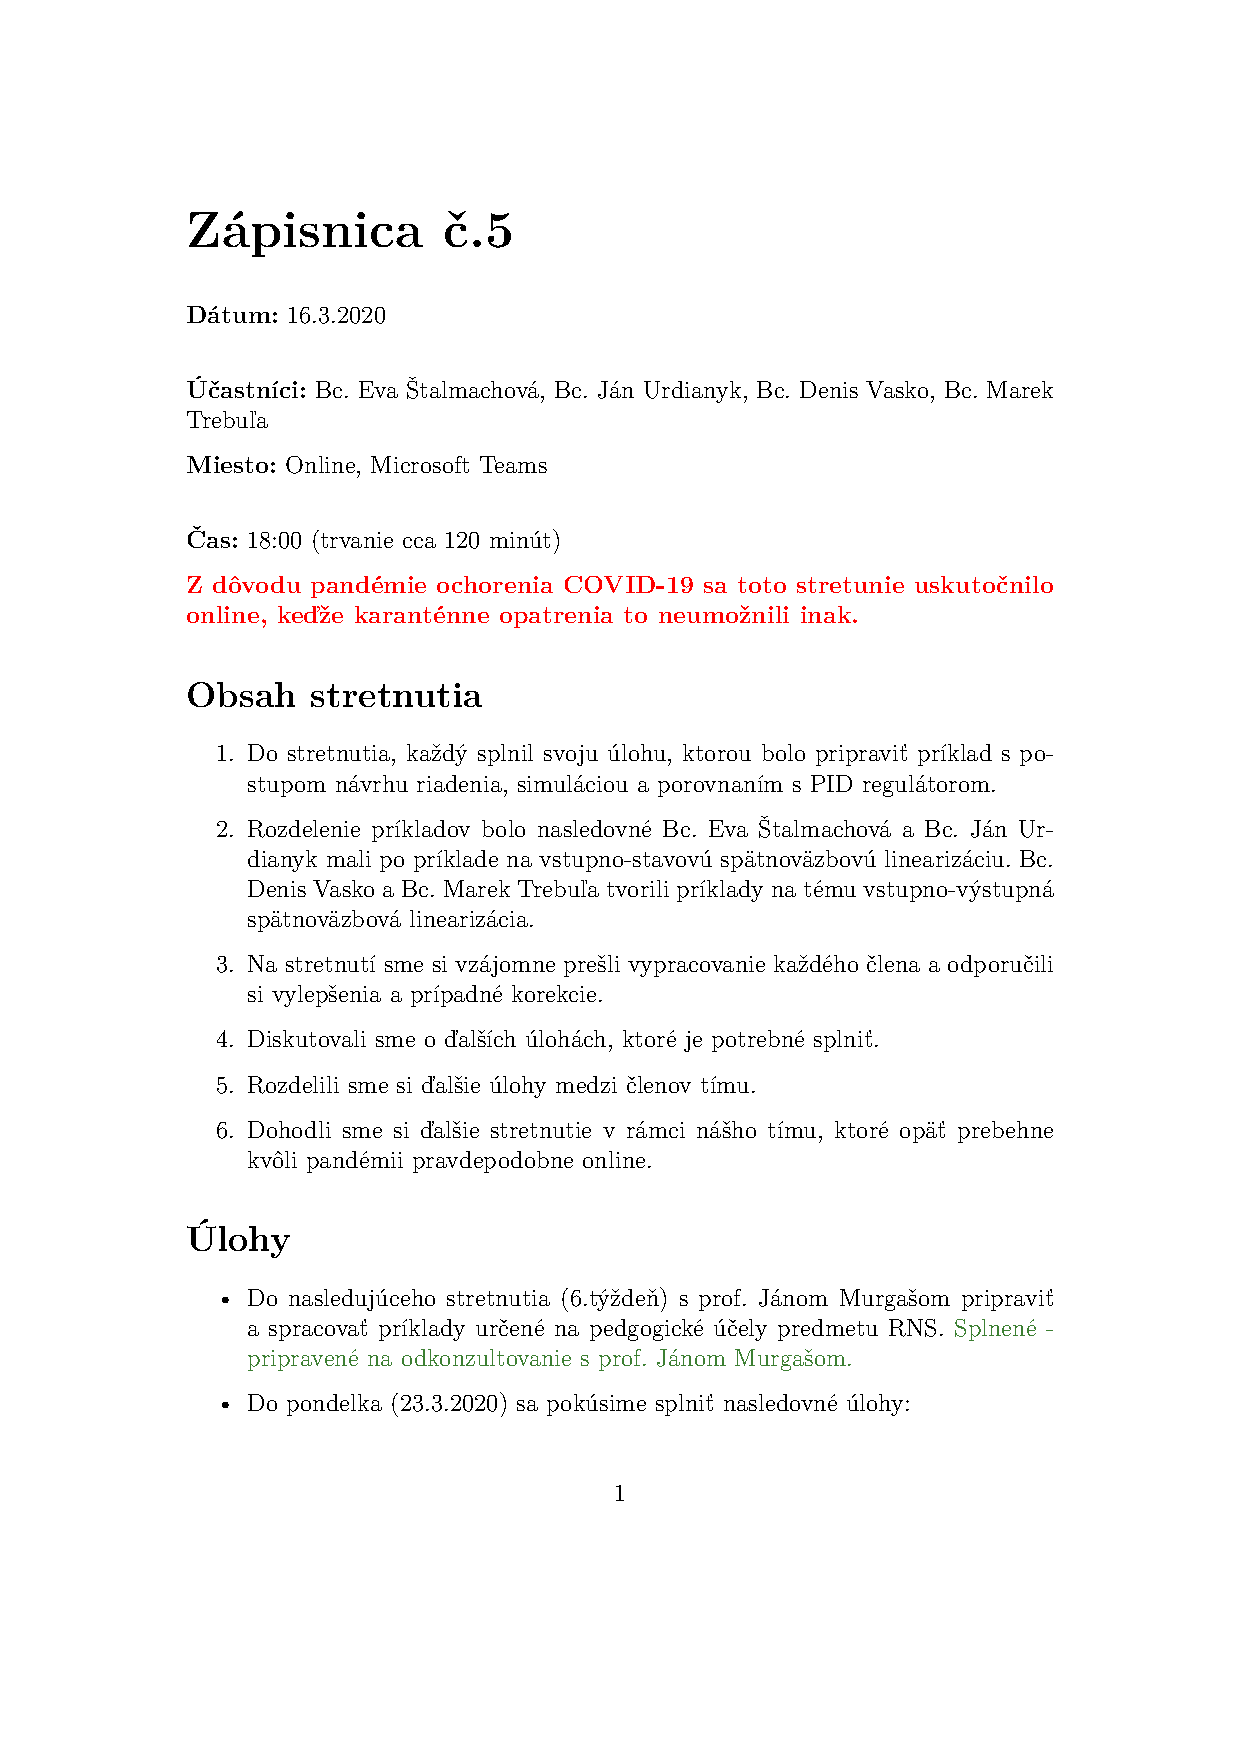
\includepdf{../../Zapisnice/Zapisnica5_16032020.pdf}
    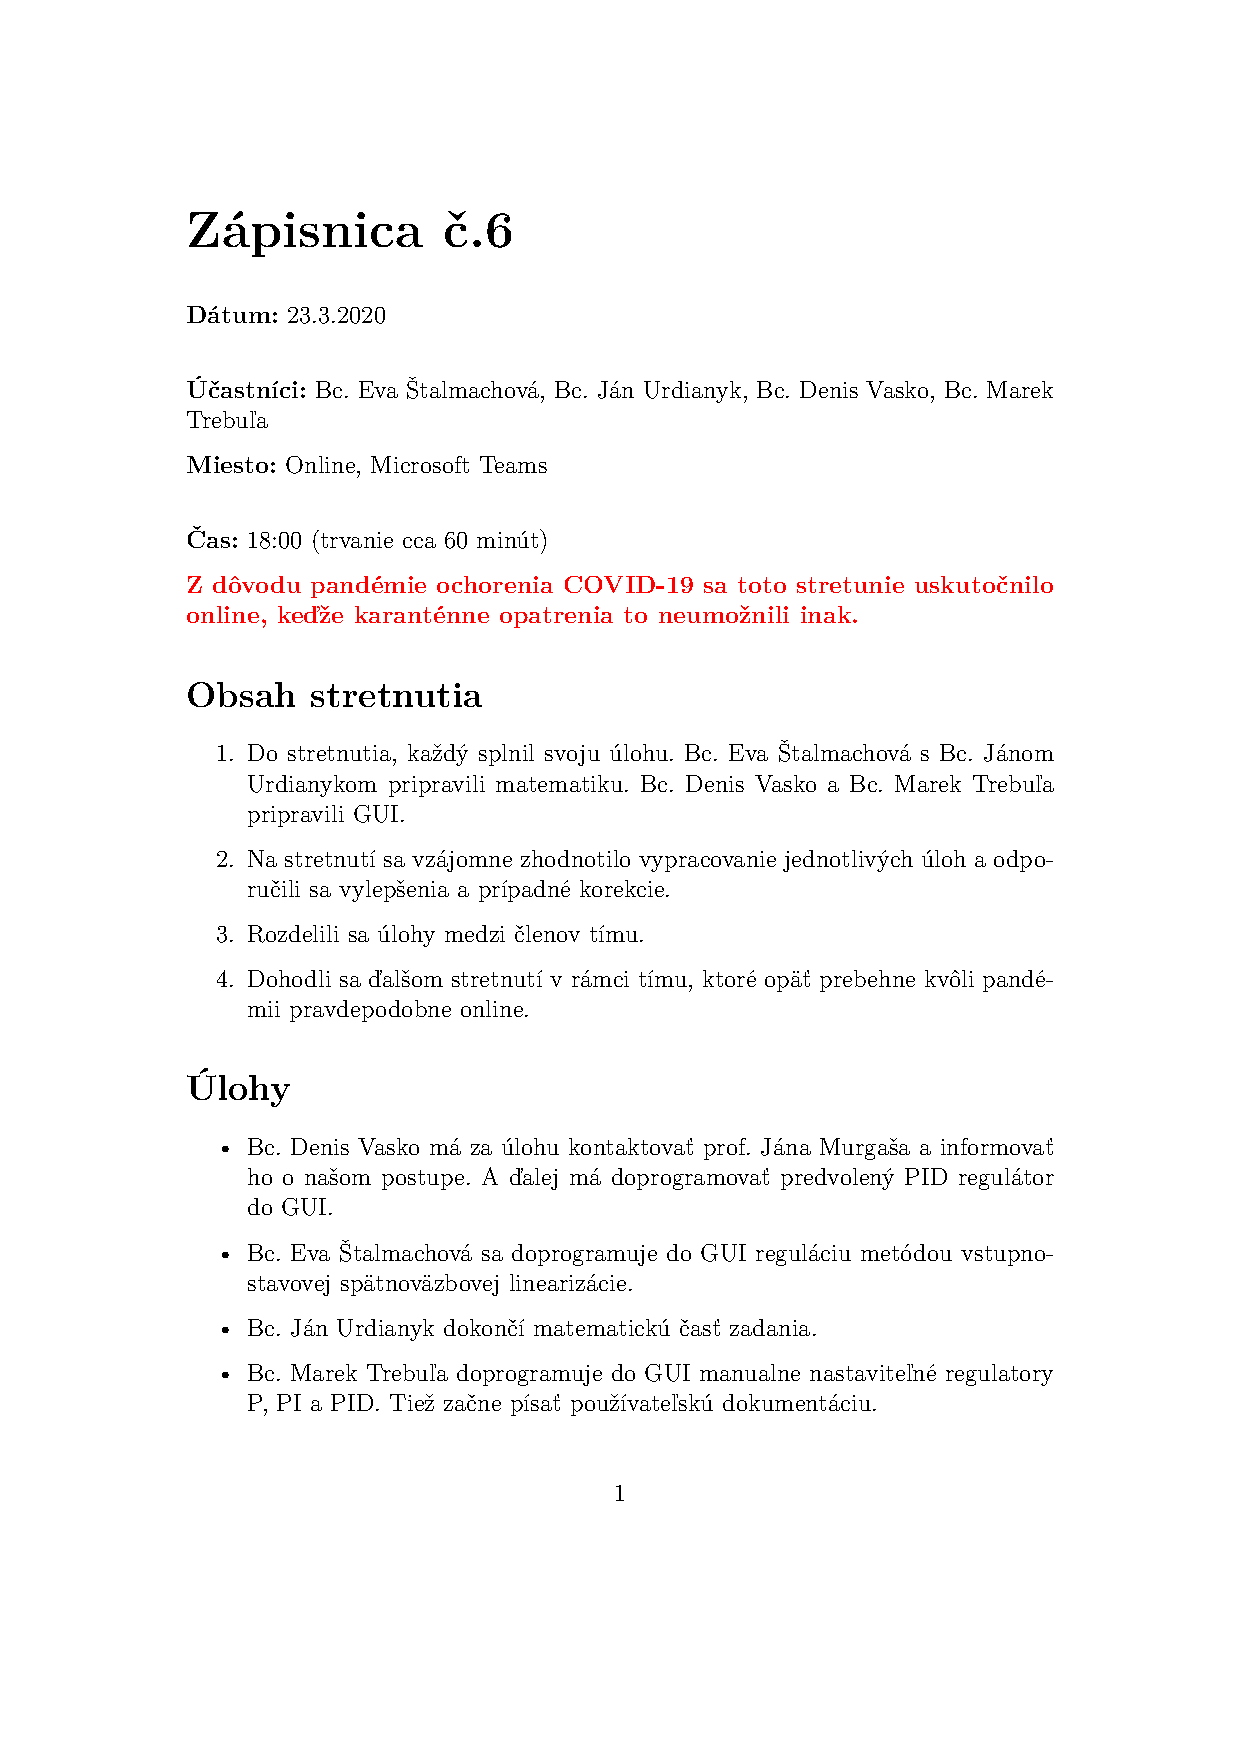
\includepdf{../../Zapisnice/Zapisnica6_23032020.pdf}
    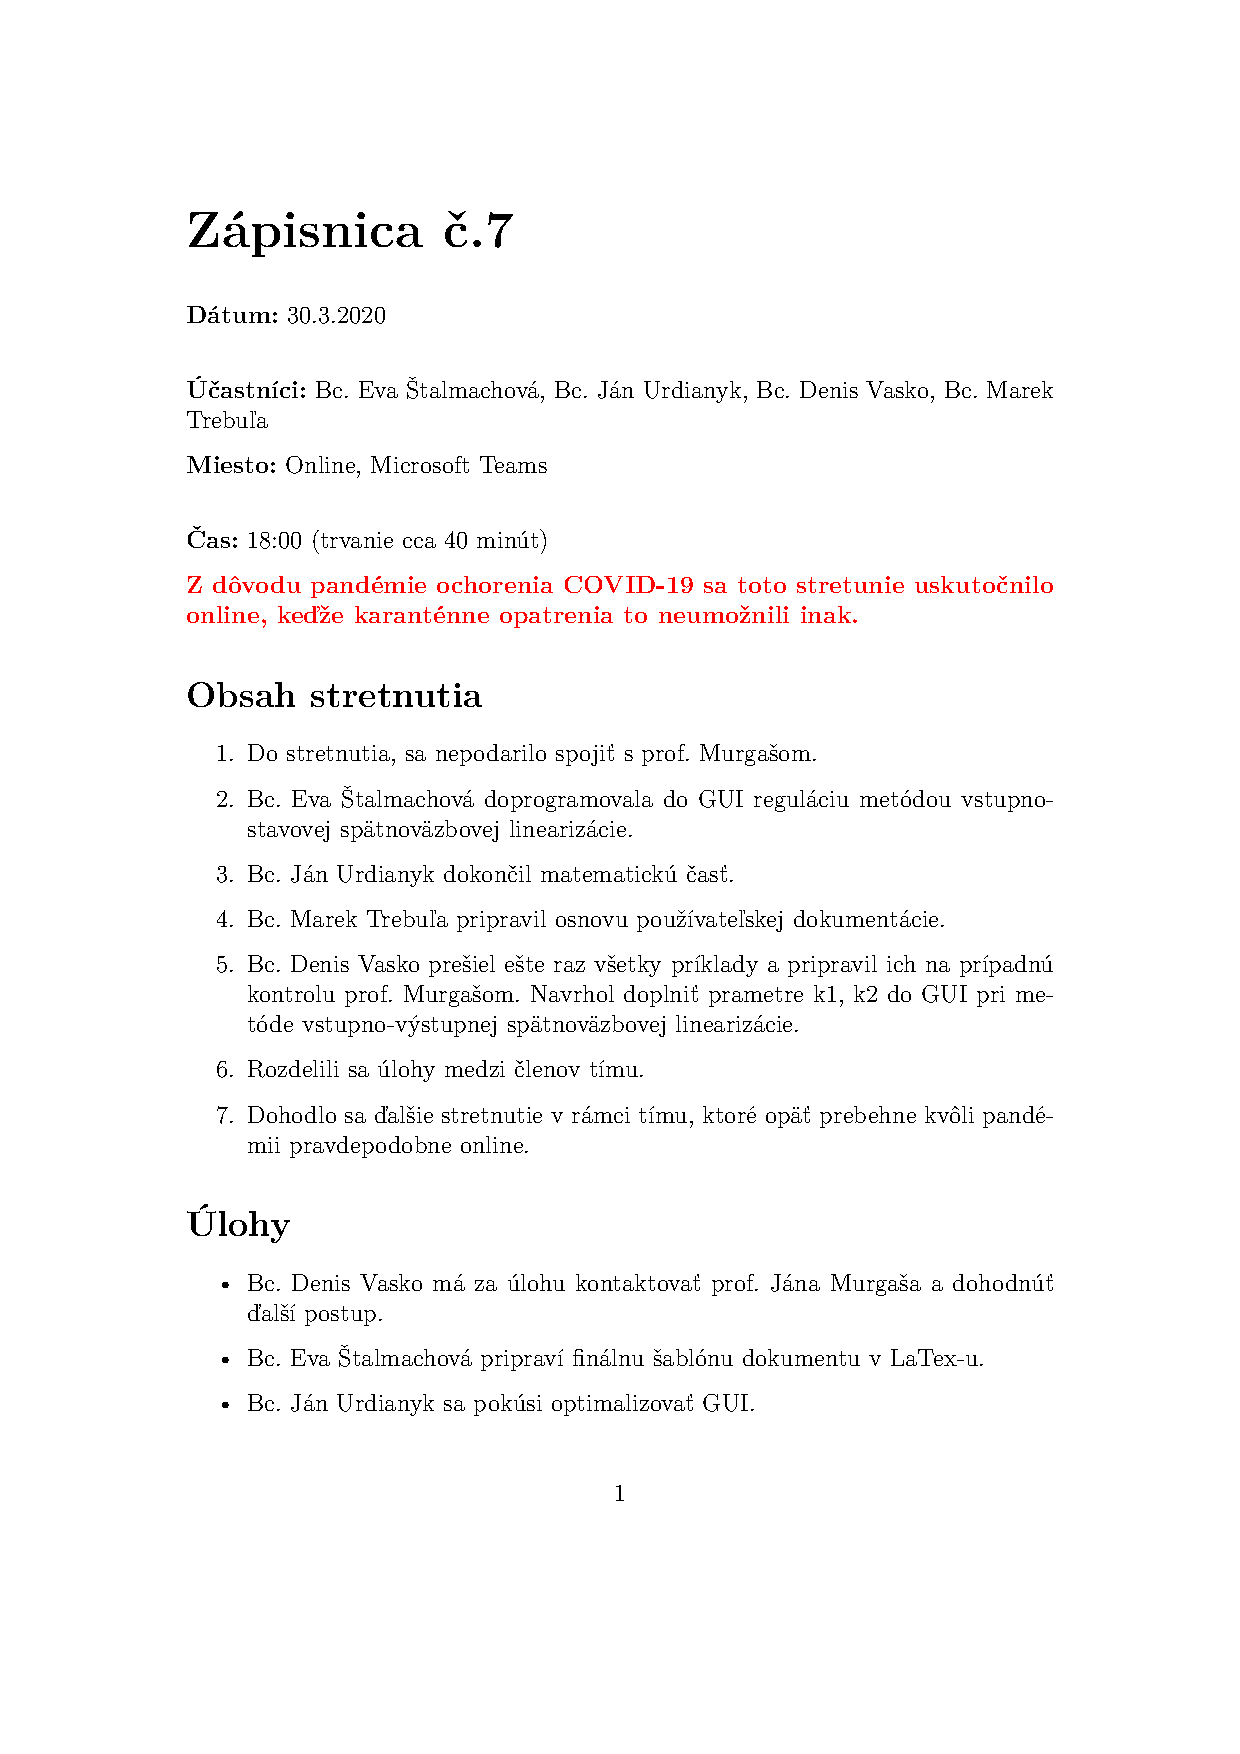
\includepdf{../../Zapisnice/Zapisnica7_30032020.pdf}
    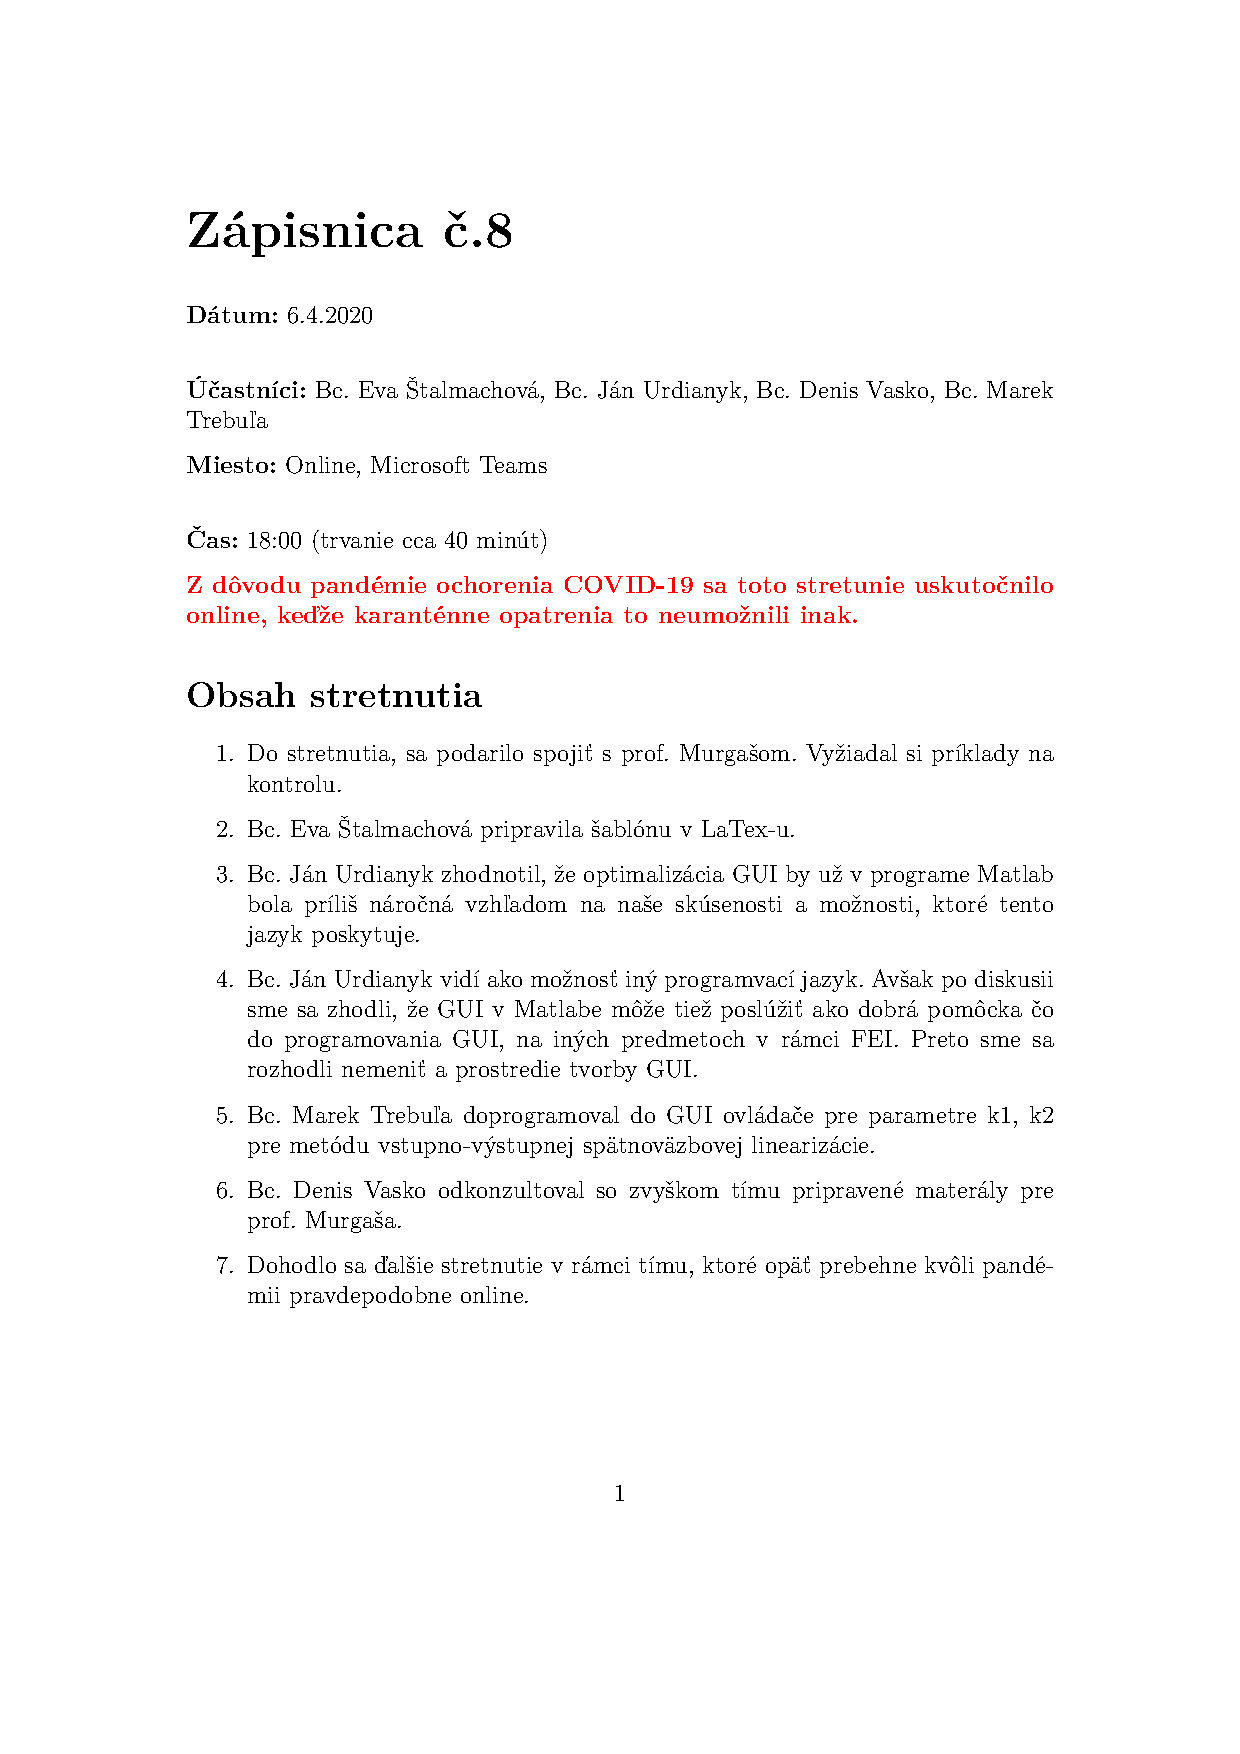
\includepdf{../../Zapisnice/Zapisnica8_06042020.pdf}
    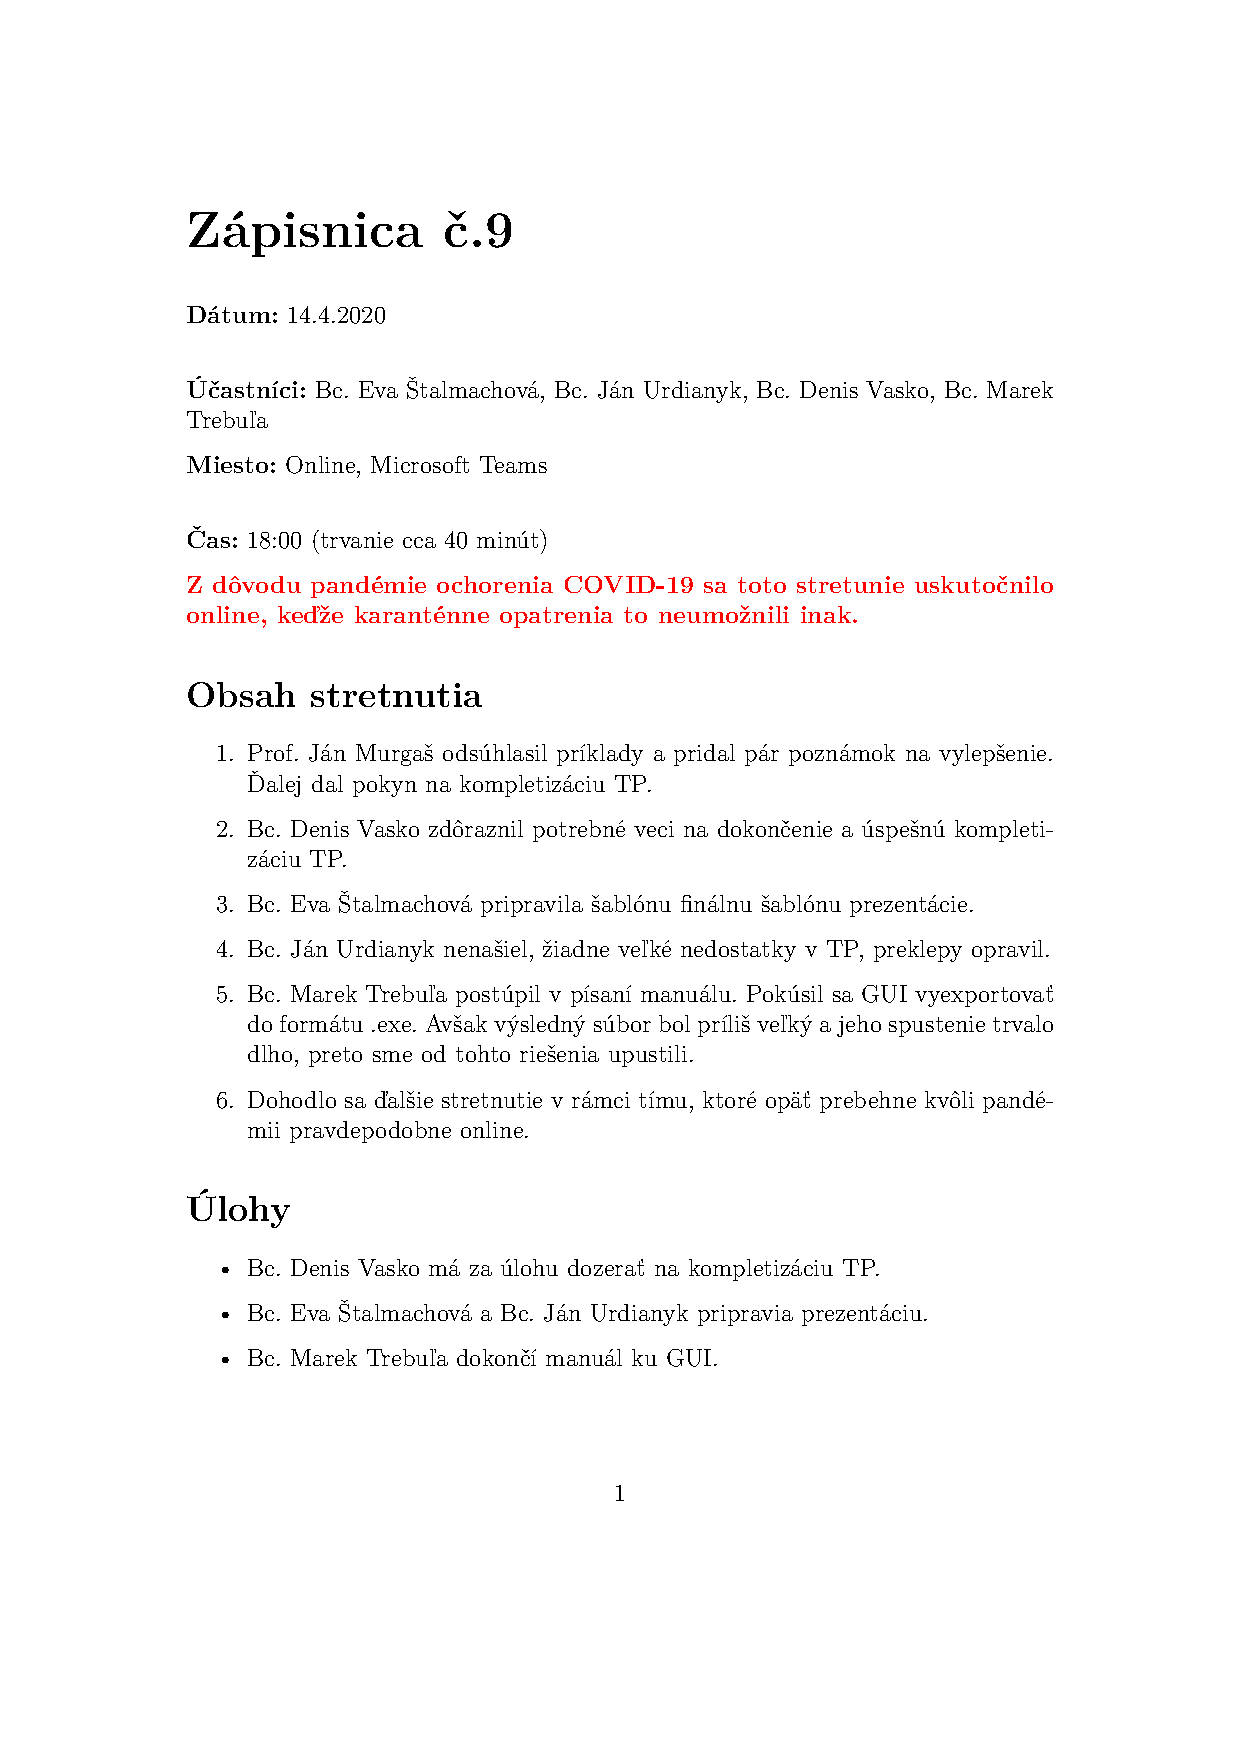
\includepdf{../../Zapisnice/Zapisnica9_14042020.pdf}
    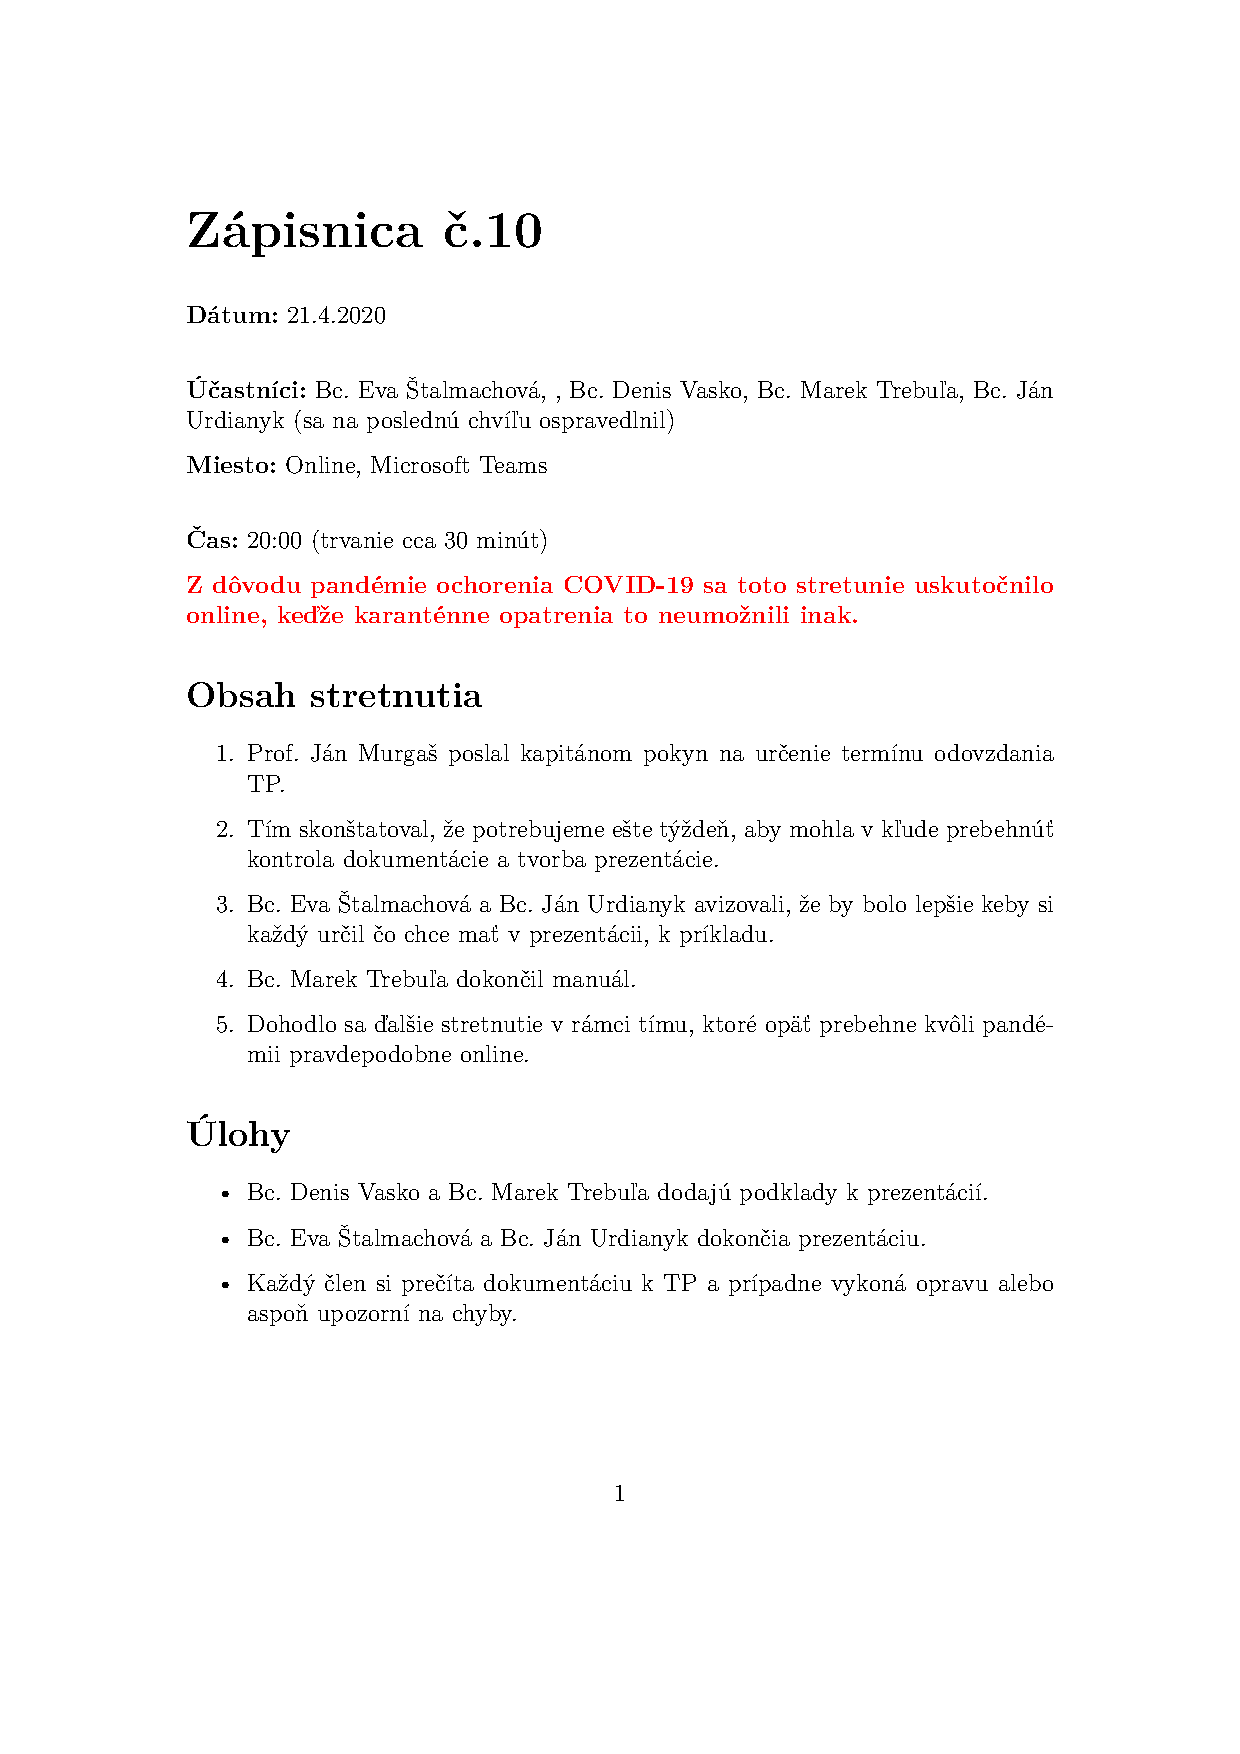
\includepdf{../../Zapisnice/Zapisnica10_21042020.pdf}

\end{document}
